% !TeX root = ../../../main.tex
\subsubsection{Geometric Constraint Primitives}%
\label{sec:solution.impl.gcps}

Having overcome the language barrier between C++ and Julia, we can build our
\ac{GC} primitives on top of \texttt{CGAL.jl}.  Our implementation follows a
constructive approach where the production of geometry can be done solely
resorting to a straightedge and a compass.  This makes programs easier to
understand and manually reproduce.

The following sections revisit of our initially formulated example problems from
\cref{sec:intro.examples}.

\subsubsection*{Parallel lines}%
\label{sec:solution.impl.gcps.parallel}

Using our \primitives{}, we devised a solution to the ``parallel lines'' problem
introduced in \cref{sec:intro.examples.parallel}.
\Cref{lst:solution.impl.gcps.parallel} shows a program combining our solution
with the Khepri \ac{AD} tool. \Cref{fig:solution.impl.gcps.parallel} illustrates
the program's output in AutoCAD\@.

\begin{listing}[htbp]
  \inputminted{julia}{jl/ex_parallel.jl}
  \caption{\label{lst:solution.impl.gcps.parallel}
    Implementation of the parallel lines example illustrated in
    \cref{fig:intro.example.parallel} using Khepri alongside our solution.}
\end{listing}

\begin{figure}[htbp]
  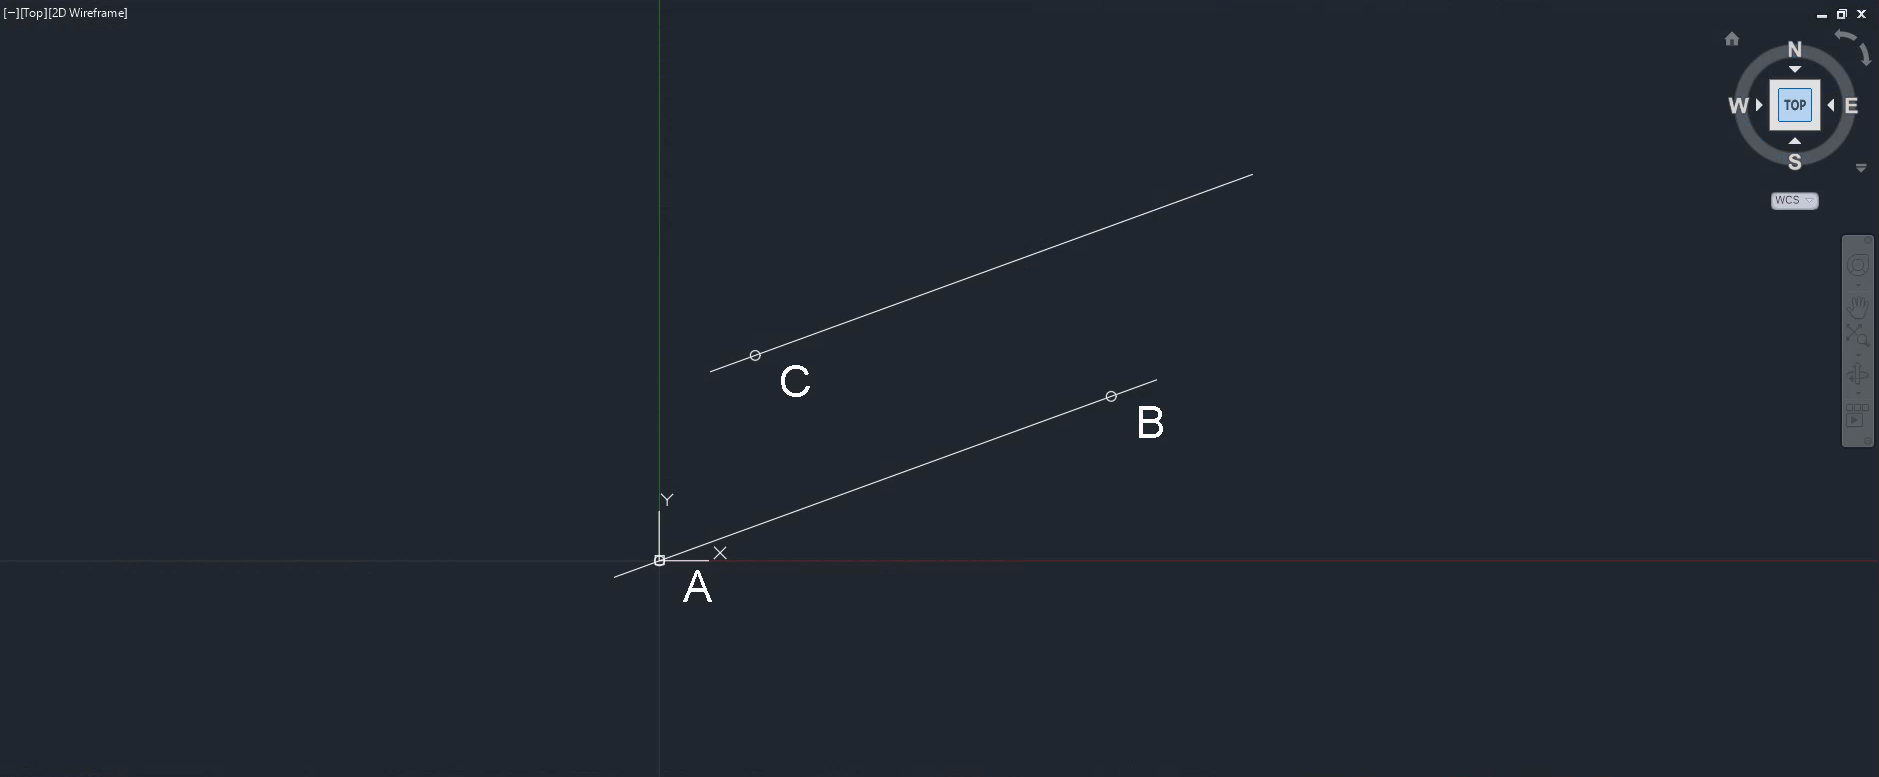
\includegraphics[width=\linewidth]{fig/autocad-parallel} 
  \caption{\label{fig:solution.impl.gcps.parallel}
    Parallel lines example using our solution, visualized in AutoCAD\@.}
\end{figure}

\subsubsection*{Circumcenter}%
\label{sec:solution.impl.gcps.circumcenter}

We initially solved the circumcenter problem by intersecting the circumscribed
triangle's bisectors.  Though we can still approach the problem that way,
defining a \texttt{circumcenter} function like the one in
\cref{lst:solution.impl.gcps.circimpl}, this functionality is already present in
\ac{CGAL},  perfectly demonstrating our approach's benefits regarding
repurposing such a comprehensive library.

\begin{listing}[htbp]
  \begin{minted}[linenos=false]{julia}
  circumcenter(a, b, c) = intersection(bisector(a, b), bisector(b, c)) 
  \end{minted}
  \caption[Initial circumcenter solution]{
    Initial implementation of \texttt{circumcenter}.}%
  \label{lst:solution.impl.gcps.circimpl}
\end{listing}

\Cref{lst:solution.impl.gcps.circumcenter} illustrates a solution to the
``circumcenter'' problem using \ac{CGAL}'s \texttt{circumcenter} function.  The
program's output can be seen in \cref{fig:solution.impl.gcps.circumcenter}.

\begin{listing}[htbp]
  \inputminted{julia}{jl/ex_circumcenter.jl}
  \caption{\label{lst:solution.impl.gcps.circumcenter}
    Implementation of the circumcenter example illustrated in
    \cref{fig:intro.example.circumcenter} using Khepri alongside our solution.}%
\end{listing}

\begin{figure}[htbp]
  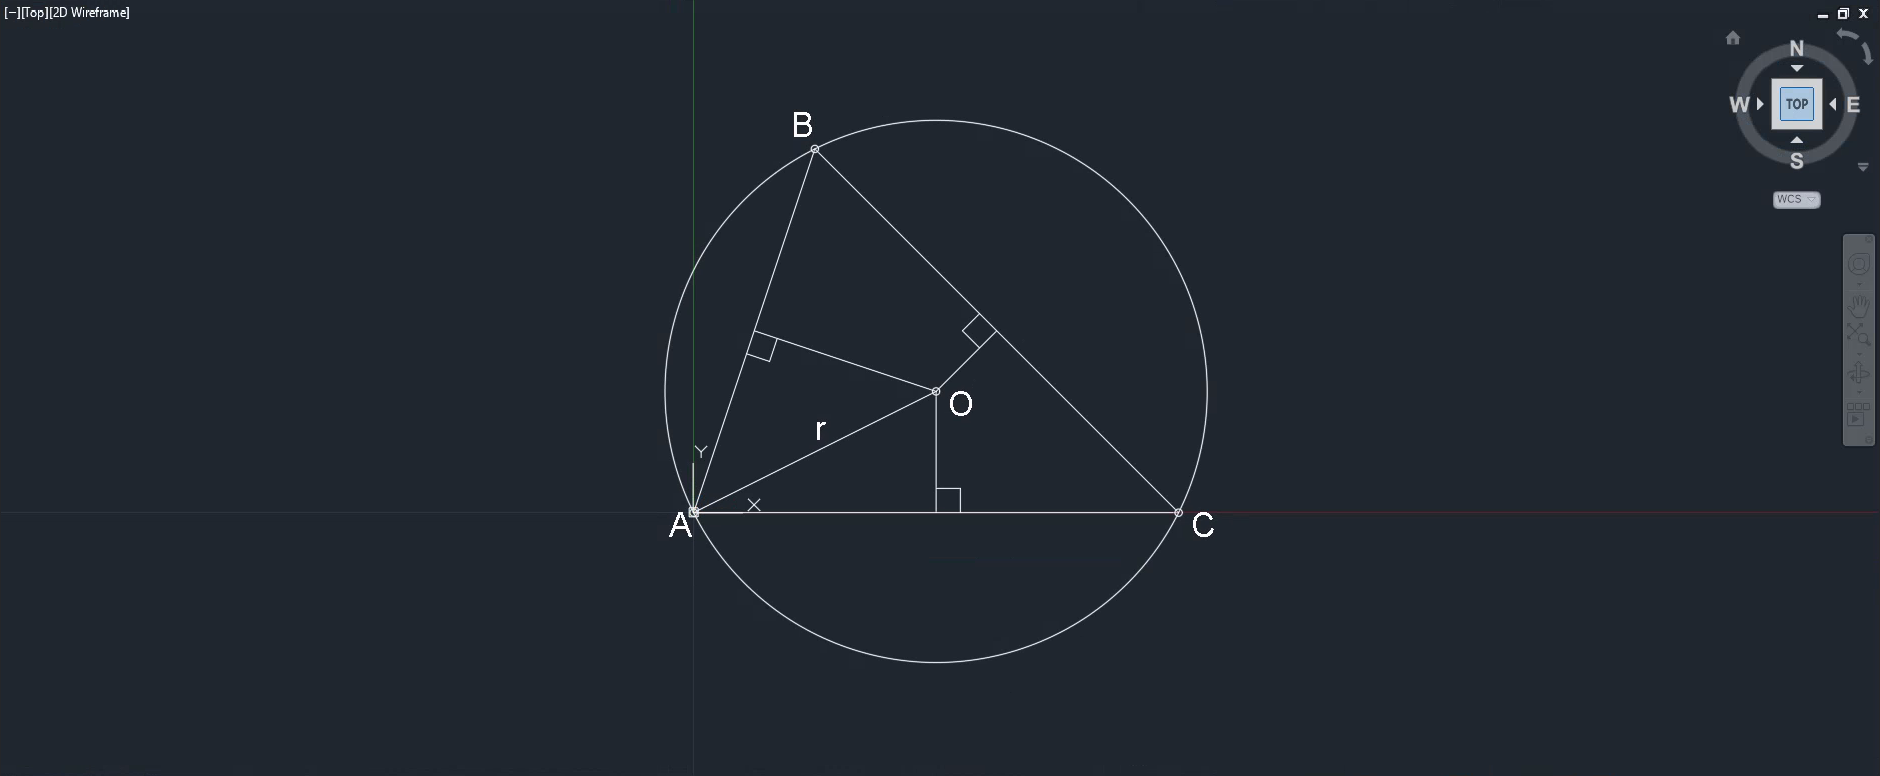
\includegraphics[width=\linewidth]{fig/autocad-circumcenter} 
  \caption{\label{fig:solution.impl.gcps.circumcenter}
    Circumcenter example using our solution, visualized in AutoCAD\@.}%
\end{figure}
